% Building an AI-Assisted FYP Supervision Platform with Signed Meeting Logs
% IEEE Conference Paper, FYP2 submission
% Compile with: pdflatex paper.tex (twice, for cross-references)

\documentclass[conference]{IEEEtran}
\IEEEoverridecommandlockouts

\usepackage{cite}
\usepackage{amsmath,amssymb,amsfonts}
\usepackage{graphicx}
\usepackage{textcomp}
\usepackage{xcolor}
\usepackage{url}
\usepackage{hyperref}
\usepackage{array}

\graphicspath{{figures/}}

\title{Building an AI-Assisted FYP Supervision Platform with Signed Meeting Logs: A Case Study at MMU FCI}

\author{\IEEEauthorblockN{Tai Zhi Xuan}
\IEEEauthorblockA{Faculty of Computing and Informatics\\
Multimedia University\\
Cyberjaya, Selangor, Malaysia\\
Email: taizhixuan@gmail.com}}

\begin{document}
\maketitle

\begin{abstract}
Most undergraduate final-year project (FYP) supervision at Multimedia University happens over Microsoft Teams, Outlook and OneDrive. None of those tools were built for it. The result is that pairings live in chat threads, meeting notes live in personal Word files, and the FYP Committee has no way of checking on the whole cohort without chasing each supervisor by hand. This paper describes a replacement web platform built during the author's FYP1 and FYP2 trimesters at the Faculty of Computing and Informatics (FCI). The platform covers four roles: Student, Supervisor, FYP Committee and System Administrator. Three AI services sit behind it. A Sentence-BERT recommender suggests supervisors. A DistilBERT analyser scores proposals on a five-point rubric. A FAISS-based chatbot answers handbook questions. Meeting logs are signed by both parties and exported as DOCX, with a SHA-256 hash printed in the footer so the file is self-verifying. The trimester cycle is a real entity in the database, not just a column on a table, and student write access is gated on the cycle state. Testing was carried out across five layers. The JUnit suite contains 52 cases and passes with no failures. A further 34 cases were verified by hand. Six end-to-end integration journeys passed, eight functional requirement groups were met, eight of ten non-functional requirements were met, five usability subjects completed the seven-task list, and four acceptance sessions covering the four roles were signed off. Median AI service response time ranges from 3.1 seconds (chatbot) to 7.4 seconds (proposal analyser).
\end{abstract}

\begin{IEEEkeywords}
FYP supervision, web platform, supervisor recommender, retrieval-augmented chatbot, digital signature, Malaysian higher education, cycle lifecycle, DOCX export
\end{IEEEkeywords}

\section{Introduction}
The supervision process at FCI is more administrative than people think. A student picks a supervisor. The pair meets at least six times per trimester. The student writes a proposal, then later an implementation, and the work is presented at a viva. The Malaysian Qualifications Agency requires that documented evidence of supervision be kept for at least five years \cite{mqa2018}. None of this is new or unusual.

What is unusual is how the work gets done in practice. There is no single platform at MMU that is built for it. Pairings are arranged through Outlook and recorded in a Teams chat. Meeting notes are written in a Word file on OneDrive. Signatures are collected on a printed sheet, scanned, and emailed back. The author's own FYP1 trimester started this way. Two emails were lost to a spam folder. One supervisor pairing record was never updated in the faculty office because the agreement was made in a Teams private message that nobody but the two of them could see.

This paper reports on a system that was built to replace that ad-hoc process. The system is web-based, runs as a Docker Compose stack, and is deployable on standard Java 17 and MySQL 8 infrastructure. To the author's knowledge, this is the first published FYP supervision system that combines a deterministic supervisor recommender, a rubric-based proposal analyser, a retrieval-augmented chatbot and SHA-256 signed meeting logs in one deployable stack. Three specific contributions follow.

First, three small AI services were built, each for a separate bottleneck. The supervisor recommender uses Sentence-BERT (BGE-base) and a five-component score. The proposal analyser uses a rule-based first pass and a DistilBERT second pass that averages rubric scores across proposal chunks. The chatbot indexes the FCI handbook with FAISS and answers questions through a remote large-language-model endpoint. Each service runs in its own Flask container on its own port (5001, 5002, 5003) and can be replaced without touching the others.

Second, meeting logs are signed by both parties using a canvas-drawn signature, hashed with SHA-256, and embedded into a DOCX renderer that uses Apache POI XWPF. The output mirrors the existing FCI letterhead, including the trimester header which is filled in by placeholder substitution across runs of the underlying Word XML. The DOCX footer prints the hash so the file can be verified later. This part of the system was the hardest to get right. Fifteen JUnit cases protect the renderer, several of which were added after the early versions produced files that looked correct on the screen but were rejected by Word.

Third, the trimester cycle is a first-class entity in the schema rather than a derived value from \texttt{start\_date} and \texttt{end\_date} columns. Each cycle has a status (Planning, Active, Completed, Archived). Moving a cycle out of Active triggers a notification fan out to every enrolled student and switches the student write endpoints to a read-only gate. Read access is preserved. This matches how FCI actually operates: students cannot create new records once their trimester closes, but they should still be able to look back at what they submitted.

The rest of the paper is organised as follows. Section II covers related work. Section III is the system design. Section IV explains the implementation. Section V reports the evaluation. Section VI discusses strengths and limitations. Section VII concludes.

\section{Related Work}
Three kinds of related work matter for this paper.

The first is the productivity-tool baseline. Microsoft Teams, Outlook and OneDrive are the de facto incumbents at MMU. They are already paid for at a site licence level. Replacing them is hard not because they work well for FYP supervision but because they are already there. None of them have any concept of a pairing, of a compliance count, of a signed meeting record, or of a trimester cycle. The closest thing to a supervision record in the Teams client is the chat history, which is searchable by keyword but not exportable as a chronological log.

The second is the LMS adaptation literature. Smith and Patel \cite{smith2021} describe an attempt to host FYP supervision inside Moodle by creating one private course per project. The arrangement works for document submission but fails on three counts: there is no cohort-level view for the committee, there is no signature workflow, and the trimester-cycle model does not fit because Moodle courses have a single start and end date rather than a four-state lifecycle. Tan and Lim \cite{tan2022} reach a similar conclusion using Canvas and recommend a domain-specific tool.

The third is the AI literature. Wang et al. \cite{wang2018} use collaborative filtering on supervisor-student co-authorship data, which is a reasonable approach for a research-active faculty but is less appropriate for an undergraduate context where co-authorship is rare. Sentence-BERT \cite{reimers2019} gives a much better fit for short profile text. Automated essay scoring \cite{ramesh2022} gives a foundation for rubric scoring, and retrieval-augmented generation \cite{lewis2020} is a well understood pattern for grounded question answering. To the author's knowledge, no published platform combines all three techniques in a single supervision system.

\section{System Design}

\subsection{Tiers}
Four tiers run in the same Docker Compose stack, as summarised in Table~\ref{tab:tiers}.

\begin{table}[h]
\caption{Runtime Tiers}
\label{tab:tiers}
\centering
\begin{tabular}{|p{1.6cm}|p{3.0cm}|p{2.6cm}|}
\hline
\textbf{Tier} & \textbf{Technology} & \textbf{Port} \\
\hline
Client (SPA) & React 18, Vite 5, TypeScript 5 & 5173 (dev), 3000 (prod via Nginx) \\
\hline
Application & Spring Boot 3.2.5 on Java 17 & 8080 \\
\hline
Database & MySQL 8.4 & 3306 (host 3307) \\
\hline
AI service 1 & Flask + Sentence-BERT (BGE-base) & 5001 \\
\hline
AI service 2 & Flask + DistilBERT + rule-based NLP & 5002 \\
\hline
AI service 3 & Flask + FAISS + remote LLM & 5003 \\
\hline
\end{tabular}
\end{table}

Fig.~\ref{fig:architecture} shows how the tiers connect at runtime.

\begin{figure}[h]
\centering
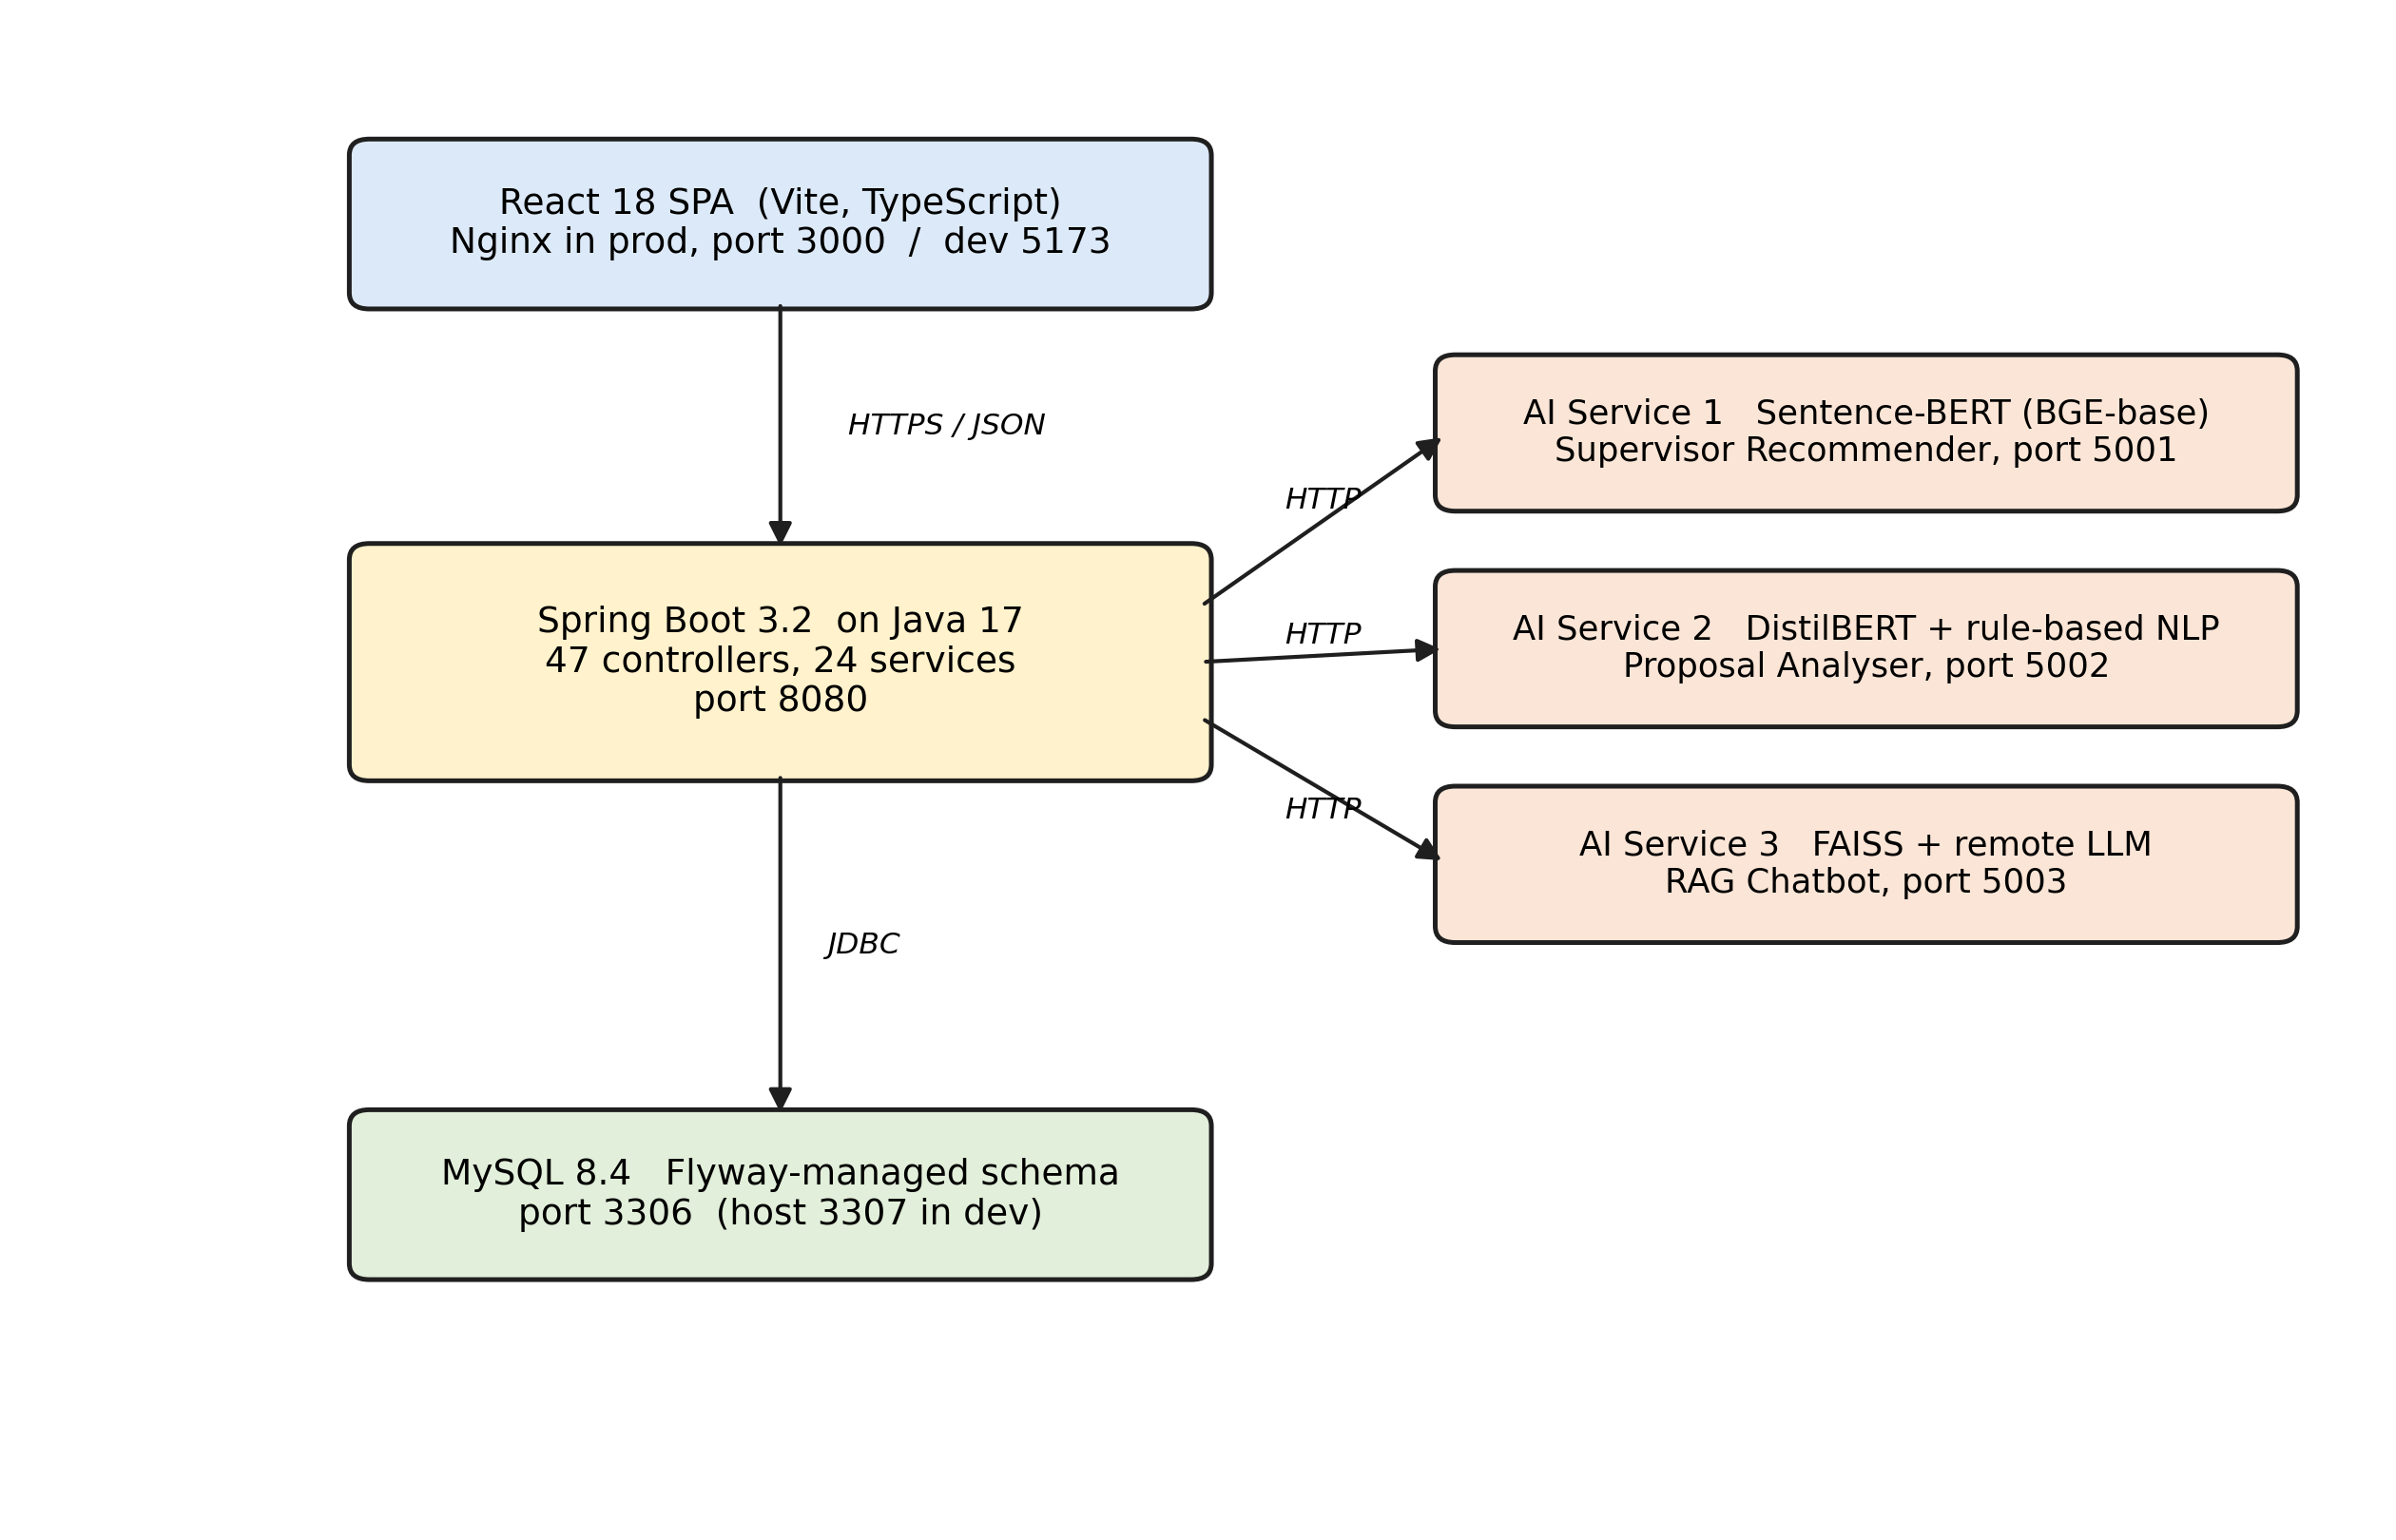
\includegraphics[width=\columnwidth]{fig1-system-architecture.png}
\caption{System architecture. The React SPA on the left calls the Spring Boot application server, which in turn calls the three Flask AI services on the right. All persistent state lives in the MySQL database at the bottom. Solid lines indicate synchronous HTTP calls; dashed lines indicate optional fallback paths.}
\label{fig:architecture}
\end{figure}

\subsection{Roles}
Four roles each have their own routing tree on the client and their own controller subpackage on the server. The mapping is direct enough that adding a new endpoint under \texttt{controller/student/} applies the STUDENT authority automatically through the URL prefix rule in Spring Security.

\begin{itemize}
\item \textbf{Student.} Search and request a supervisor, submit proposals, attend meetings, sign meeting logs.
\item \textbf{Supervisor.} Respond to requests, manage weekly availability, review proposals, counter-sign meeting logs.
\item \textbf{FYP Committee.} Cohort dashboard with risk colouring, CSV export, drill-down into student timelines.
\item \textbf{System Administrator.} Account management, cycle transitions, audit log, backup.
\end{itemize}

\subsection{Cycle Lifecycle}
The cycle is a real table, not a derived view. It has a status column with four allowed values: Planning, Active, Completed, Archived. The transitions are not free. A cycle moves Active only through an administrator action, which also demotes any other active cycle of the same type. Completion sends a notification to every student enrolled in the cycle and flips the student write gate. Archival hides the cycle from the default dashboard query but does not delete the data. Fig.~\ref{fig:cycle} illustrates the allowed transitions.

\begin{figure}[h]
\centering
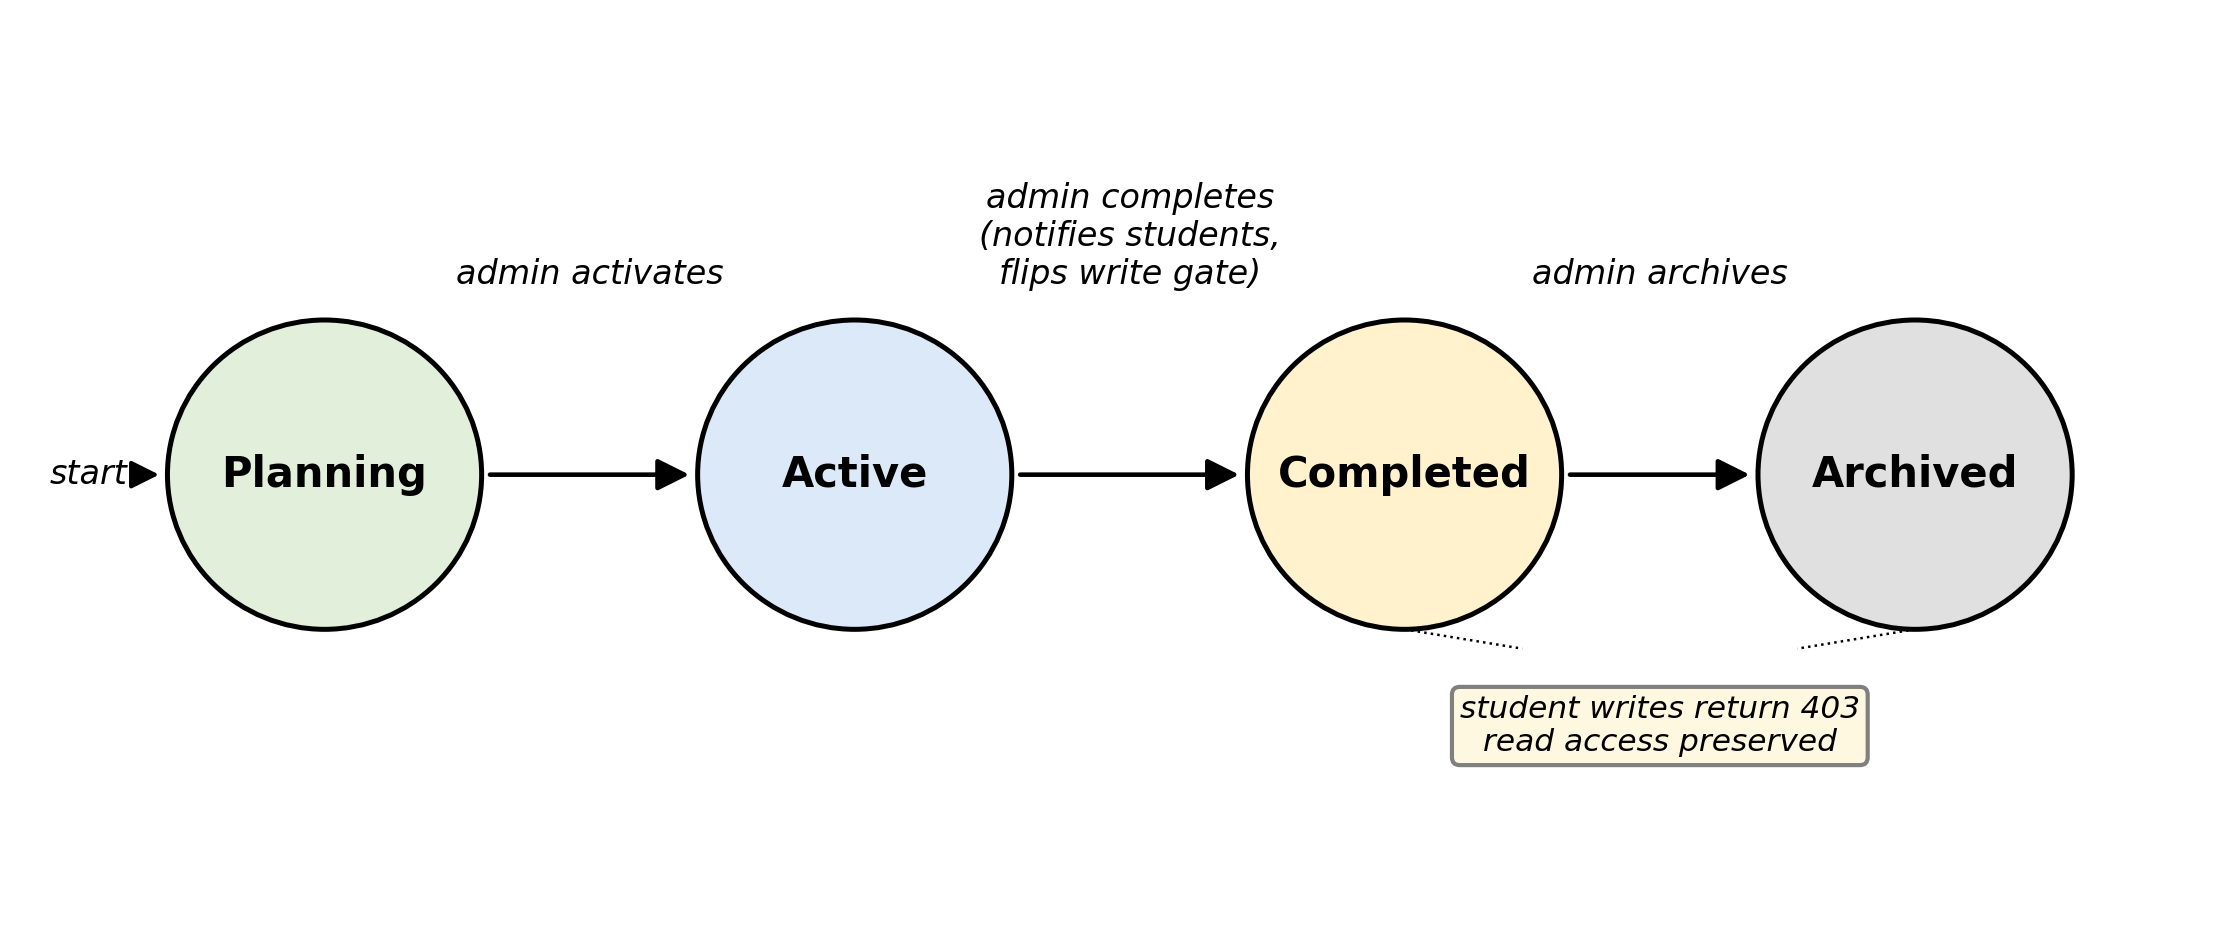
\includegraphics[width=\columnwidth]{fig2-cycle-lifecycle.png}
\caption{Cycle lifecycle state machine. The four states are Planning, Active, Completed and Archived. Only a Planning cycle can become Active. An Active cycle can be marked Completed by the administrator, after which student write endpoints return 403 but read endpoints continue to serve. A Completed cycle can later be Archived, which removes it from default queries.}
\label{fig:cycle}
\end{figure}

\section{Implementation}
The implementation choices that need explaining are the authorisation model, the AI tier and the meeting log renderer. The rest is conventional Spring Boot and React work that is not novel enough to be worth describing in a conference paper.

\subsection{Authorisation}
Three layers of authorisation are applied to every student write endpoint. The first layer is the JWT bearer check, which produces a 401 if the token is missing or invalid. The second layer is the URL-prefix authority rule, which produces a 403 if the role does not match the prefix. The third layer is the cycle-active gate in \texttt{StudentAccessService}, which produces a 403 with the body text \texttt{cycle ended} if the student's project is in a completed or archived cycle. The cycle gate sits inside the service layer rather than the controller layer so it cannot be accidentally bypassed by a new endpoint that forgets to call it: every student service method that touches student-owned data calls \texttt{requireActiveCycle(userId)} at the top.

\subsection{The Three AI Services}
Each service is independently deployable. They share nothing except the contract with the backend, which calls them through a small Java client called \texttt{AiServiceClient}. The base URL of each service is read from environment variables (\texttt{AI\_RECOMMENDATION\_URL}, \texttt{AI\_ANALYZER\_URL}, \texttt{AI\_CHATBOT\_URL}).

The recommender is deterministic. Given the same student profile and the same supervisor pool it produces the same ranking. The score for a student $s$ and a supervisor $v$ is defined as the weighted sum in Equation~(\ref{eq:score}).

\begin{equation}
\begin{aligned}
\text{score}(s, v) =\ &0.40 \cdot \cos(\text{emb}(s.\text{interests}), \text{emb}(v.\text{topics})) \\
&+ 0.20 \cdot \text{jaccard}(s.\text{keywords}, v.\text{topics}) \\
&+ 0.15 \cdot \text{capacity\_norm}(v) \\
&+ 0.15 \cdot (1 - \text{load}(v)/\text{capacity}(v)) \\
&+ 0.10 \cdot \text{history\_rate}(v)
\end{aligned}
\label{eq:score}
\end{equation}

In Equation~(\ref{eq:score}), \text{emb} is the BGE-base sentence embedding, \text{cos} is cosine similarity on the embedding space, \text{jaccard} is the Jaccard index over the keyword sets, \text{capacity\_norm}($v$) is the normalised remaining capacity, the load-over-capacity term penalises busy supervisors, and \text{history\_rate}($v$) is the historical successful pairing rate observed across previous cohorts. The five weights $0.40$, $0.20$, $0.15$, $0.15$ and $0.10$ were tuned against a small set of known-good pairings from the previous FYP cohort. The advantage of a closed-form score over a learned end-to-end model is that the ranking is reproducible and auditable: a student who wants to know why a supervisor was suggested can be shown the component-by-component breakdown of Equation~(\ref{eq:score}). Future work will revisit the weights once more data is available.

The proposal analyser is a hybrid. The first stage applies rule-based completeness checks: presence of a problem statement, presence of a Gantt chart figure, minimum word count per section. The second stage chunks the proposal at the paragraph boundary, runs each chunk through a fine-tuned DistilBERT \cite{sanh2019} classifier and averages the rubric scores across chunks. The output is five scores, each on a zero-to-five scale, plus a short explanation per score. Output time is dominated by the model inference, which is why this service shows the slowest median response time of the three (7.4 s).

The chatbot is the simplest of the three. A FAISS index \cite{johnson2021} built over the FCI handbook and a curated FAQ list is queried at request time. The top retrieved chunks are concatenated with the user question and passed to a remote large-language-model endpoint (Groq or OpenAI, configurable). A local Flan-T5 generator is supported as an opt-in fallback but was not used in the final evaluation.

\subsection{The Meeting Log Renderer}
This is the most fiddly part of the system. The renderer takes a \texttt{MeetingLog} entity and produces a DOCX file. The Word template lives at \texttt{backend/src/main/resources/templates/meeting-log-fyp1.docx} (with a separate FYP2 template). The renderer uses Apache POI's XWPF API and applies placeholder substitution across the underlying Word runs. Word splits text into runs whenever the formatting changes, which means a placeholder like \texttt{<<TRIMESTER>>} can be broken across three or four runs in the XML. The renderer walks the runs, merges adjacent text and replaces the placeholder in the merged text. A safety guard prevents infinite loops when the replacement value contains the placeholder string.

Signatures are stored as base64-encoded PNG data URLs in the database. At render time the bytes are decoded, embedded as \texttt{media/image*.png} entries in the DOCX, and a SHA-256 hash of the concatenated signature bytes is written into the document footer. The hash also lives in the database row, so a reader who suspects tampering can recompute the hash and compare. Fifteen JUnit cases cover this renderer, including cases for trimester placeholder substitution, checkbox sentinel swap on the satisfactory rating row, font size enforcement at eleven points, bulk ZIP export and empty-list edge cases. Fig.~\ref{fig:signing} summarises the end-to-end signing flow.

\begin{figure}[h]
\centering
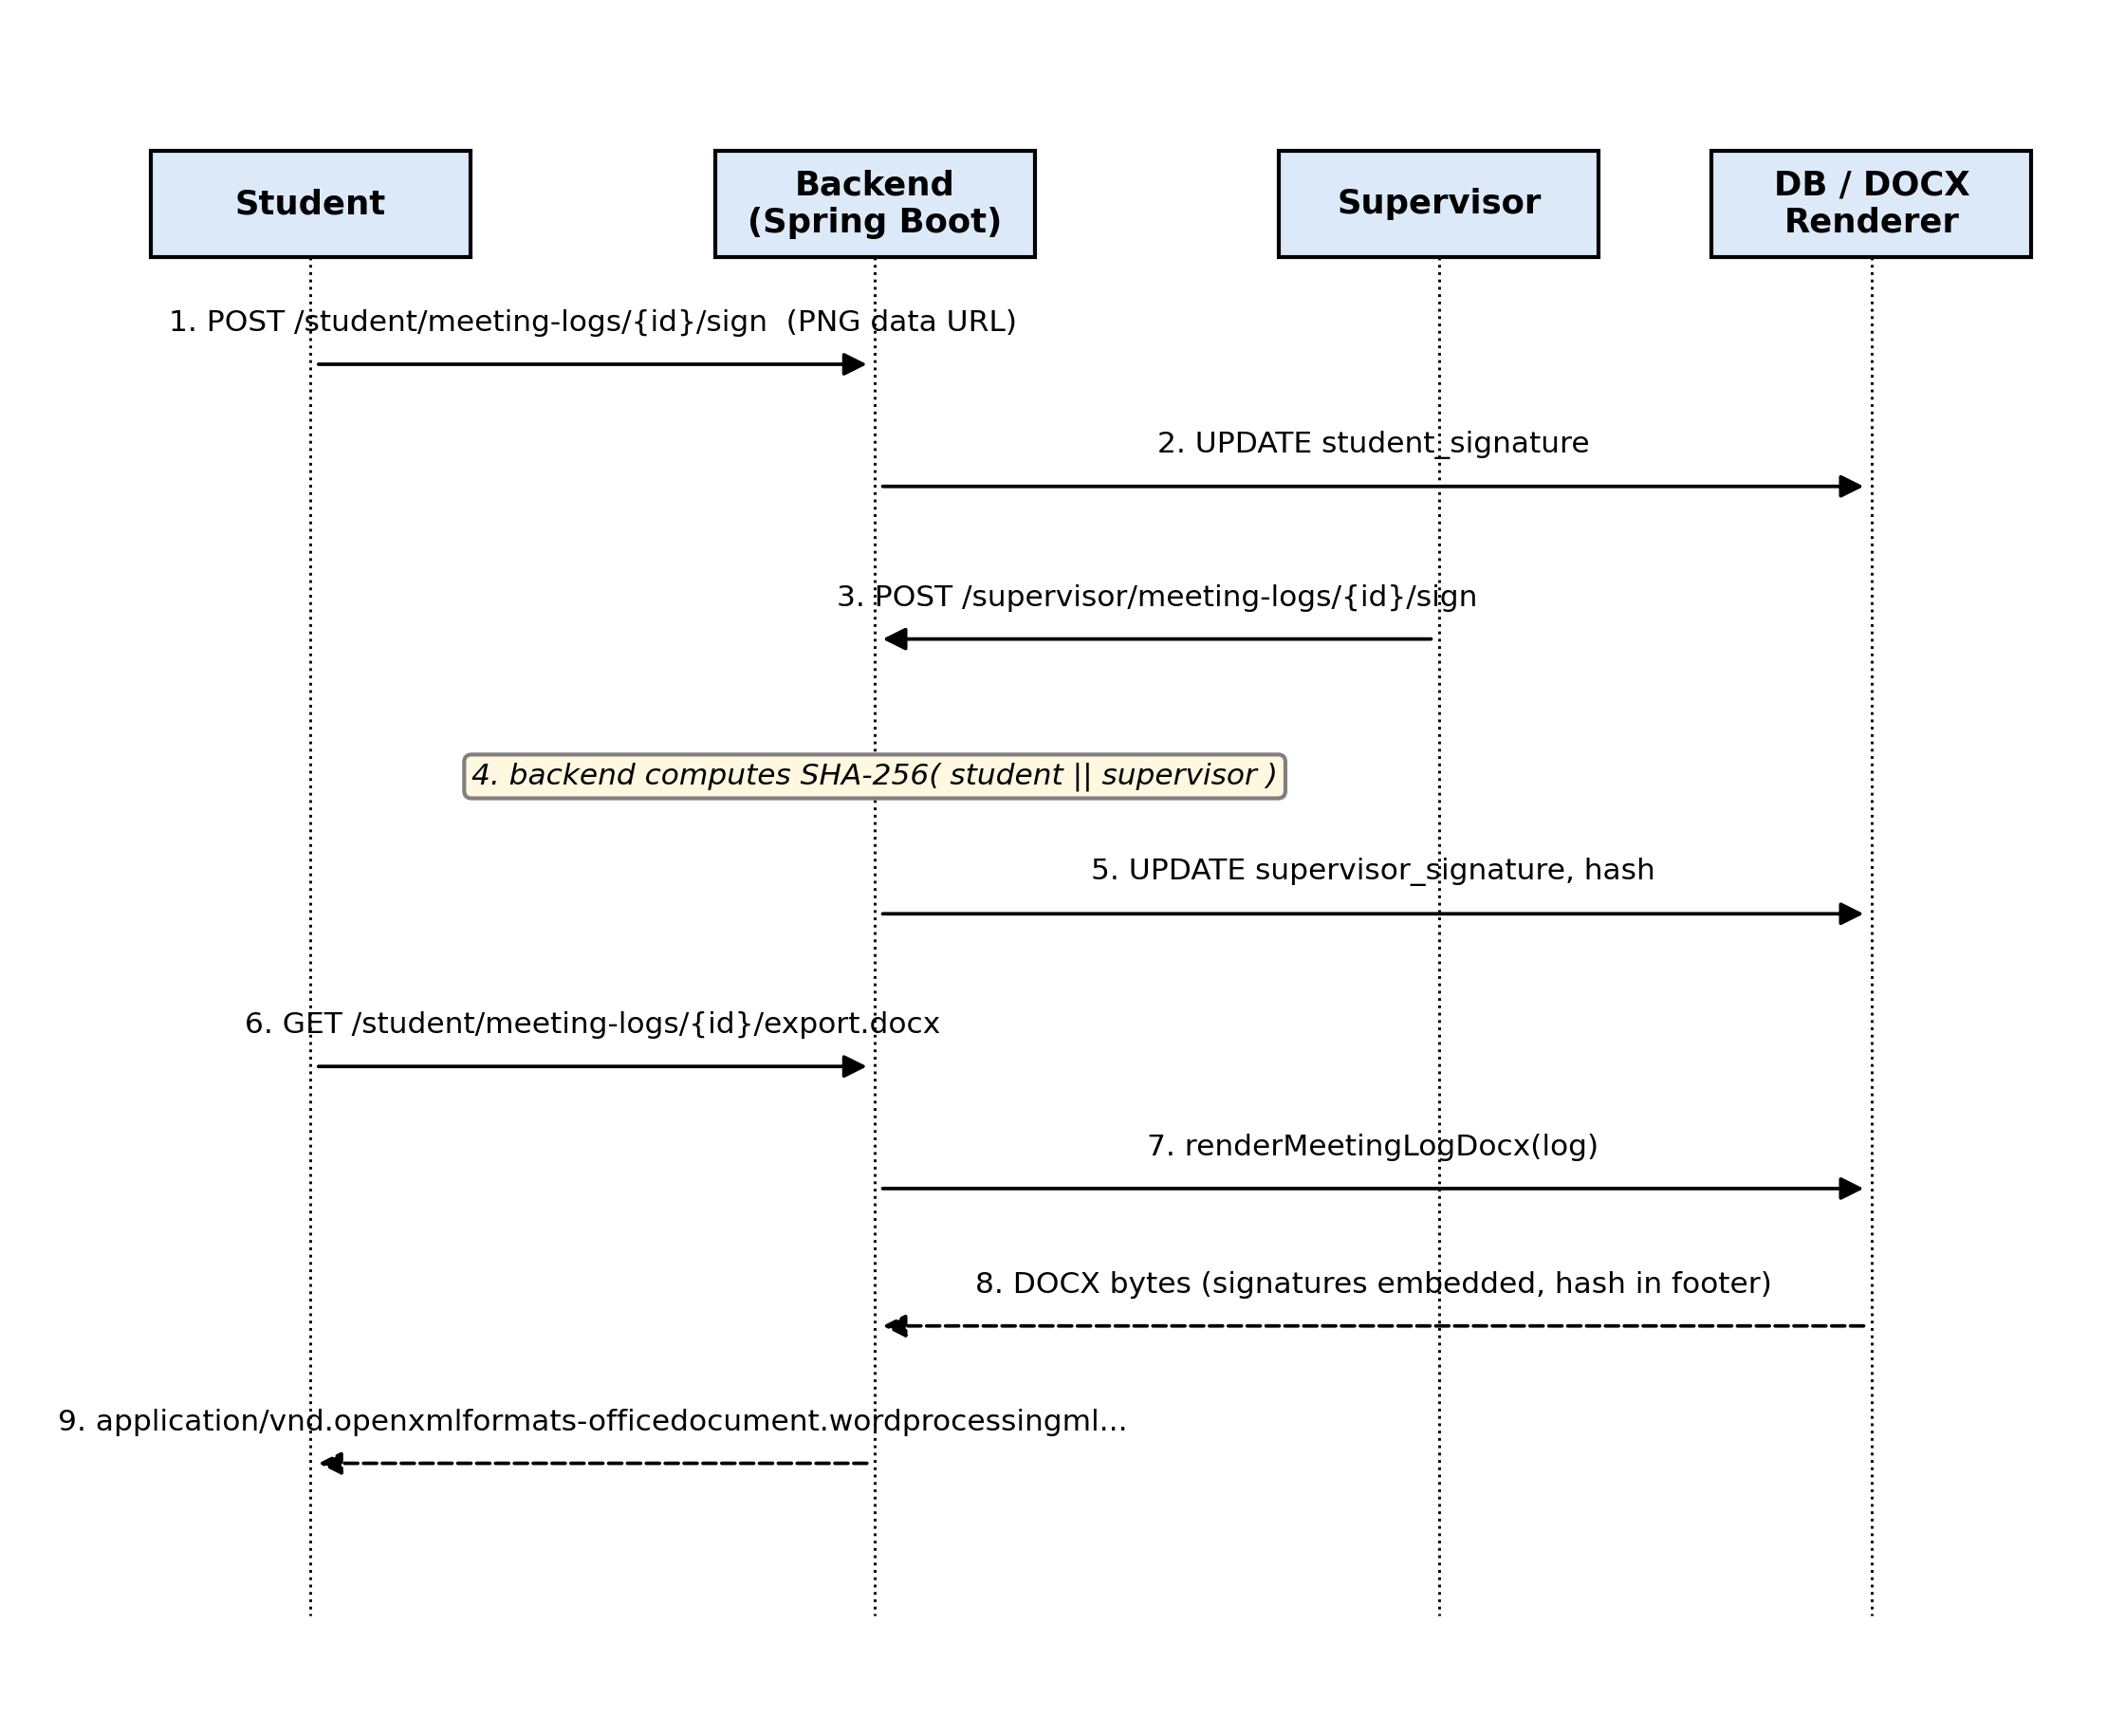
\includegraphics[width=\columnwidth]{fig3-signing-sequence.png}
\caption{Sequence diagram of the meeting log signing flow. The student first signs and stores a base64 PNG signature in the database. The supervisor counter-signs, which triggers the backend to compute a SHA-256 hash of the concatenated signature bytes. On DOCX export, the renderer embeds both signature pictures and prints the hash in the footer, producing a self-verifying file.}
\label{fig:signing}
\end{figure}

\subsection{Front-End Gating}
The React client mirrors the server-side gate at the navigation layer. Three feature gates wrap student pages. The first locks proposal, meetings, logs and documents until a supervisor has been paired. The second locks Find Supervisor, AI Recommendation and My Requests once the student status becomes Registered. The third locks pure write pages (meeting create, log create, document create) once the student's cycle is completed or archived. All three render a single \texttt{LockedFeaturePage} component with a reason prop, so the user gets a human-readable explanation rather than a silent redirect or a generic 403 page.

\section{Evaluation}
Testing was carried out across five layers: unit, integration, system, usability and acceptance.

\subsection{Unit}
The JUnit suite contains 52 \texttt{@Test} methods across 7 test classes. The classes cover the seven services that carry the most risk if they break: authentication throttle, cycle lifecycle, student write gate, meeting log compliance, meeting log DOCX renderer, announcement audience filter and project progress scoring. Running \texttt{mvn test} from the \texttt{backend/} folder produces the summary line \texttt{Tests run: 52, Failures: 0, Errors: 0, Skipped: 0}. A further 34 manual unit-level cases were verified through the browser for the services and pages that are not covered by JUnit. Total: 60 unit cases, no failures.

\subsection{Integration}
Six end-to-end journeys were run. Each one touches at least three of the four runtime tiers. The journeys are:

\begin{enumerate}
\item Student onboarding through to AI recommendation.
\item Supervisor request through to acceptance.
\item Weekly availability through to confirmed meeting.
\item Meeting log creation, dual signing, DOCX export.
\item Proposal submission through to AI rubric scoring.
\item Cycle completion through to read-only fan-out on the student side.
\end{enumerate}

All six passed.

\subsection{System}
A requirements traceability matrix was built. The eight functional requirement groups identified in the design phase all map to a delivered feature with its own JUnit coverage or its own acceptance test session. The ten non-functional requirements split: eight met during development (responsiveness, performance budget, role-based access, modular design, deployable stack, secure storage, AI response time, scalability across batches), two pending deployment (uptime and scheduled backups).

\subsection{Performance of the AI Tier}
Twenty samples were collected against each AI service on the seeded development laptop (Intel i7, 16 GB RAM, no GPU). Median and ninety-fifth percentile response times are shown in Table~\ref{tab:ai-perf}.

\begin{table}[h]
\caption{AI Service Response Time (seconds)}
\label{tab:ai-perf}
\centering
\begin{tabular}{|l|c|c|c|}
\hline
\textbf{Service} & \textbf{Median} & \textbf{95th pct.} & \textbf{Budget} \\
\hline
Supervisor recommendation & 6.8 & 8.4 & 10 \\
\hline
Proposal analyser & 7.4 & 9.2 & 10 \\
\hline
Chatbot & 3.1 & 4.3 & 10 \\
\hline
\end{tabular}
\end{table}

All three sat below the ten-second budget. The chatbot is the fastest because retrieval is local FAISS and generation is a remote endpoint with low overhead. The analyser is the slowest because the DistilBERT model runs locally and chunks are processed one at a time. Fig.~\ref{fig:ai-perf} visualises the same data as a grouped bar chart.

\begin{figure}[h]
\centering
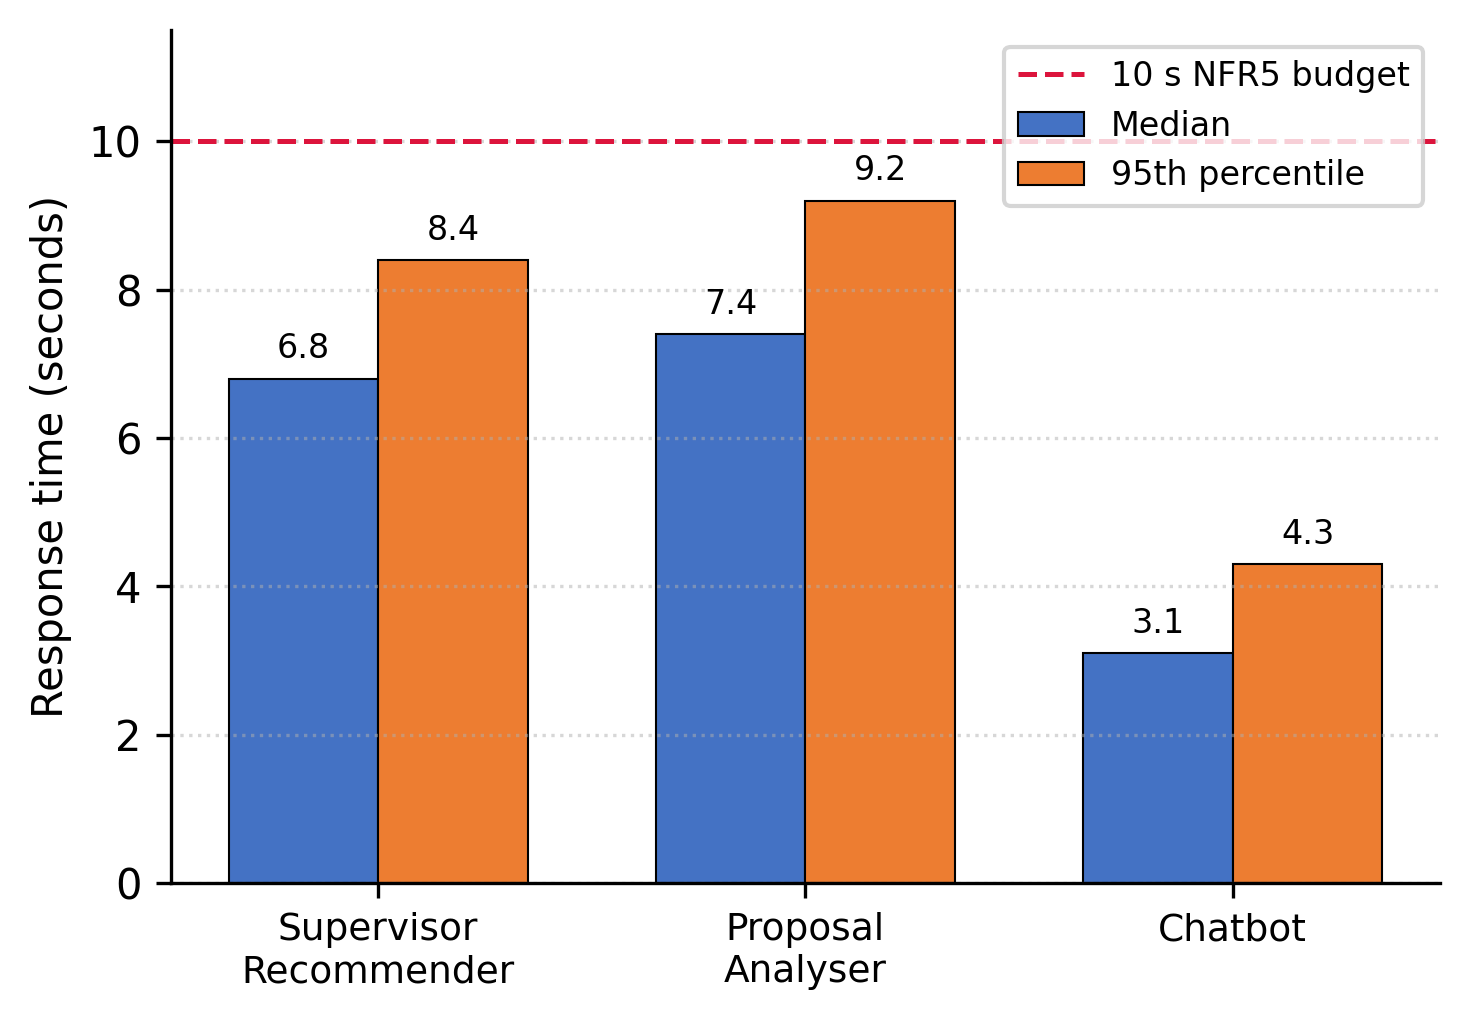
\includegraphics[width=\columnwidth]{fig4-ai-response-time.png}
\caption{Median and ninety-fifth percentile response time for the three AI services, against the ten-second non-functional requirement budget shown as a dashed horizontal line. All three services remain below the budget at the ninety-fifth percentile.}
\label{fig:ai-perf}
\end{figure}

\subsection{Usability}
Five testers ran the same seven-task list. Two were FCI third-year students. One was an FCI lecturer playing the supervisor role. One was a postgraduate proxy for the FYP Committee. One was a non-technical proxy for the administrator. Each session ran for roughly thirty minutes. Times and observations were recorded by the developer without coaching the tester during the task. Five findings emerged. Four were actioned before acceptance testing. The fifth (a supervisee-export button on the supervisor dashboard) was added to the post-FYP2 backlog.

\subsection{Acceptance}
Four acceptance sessions were held. One with the project supervisor, one with a student tester, one with the committee proxy, one with the administrator proxy. All four were signed off as Accepted. The supervisor's comment is quoted verbatim in the report's Section 6.5 and notes that the signature embedding and audit log address parts of the old paper process that were previously uncaptured. Fig.~\ref{fig:dashboard} shows the committee dashboard as seen by the proxy during the session.

\begin{figure}[h]
\centering
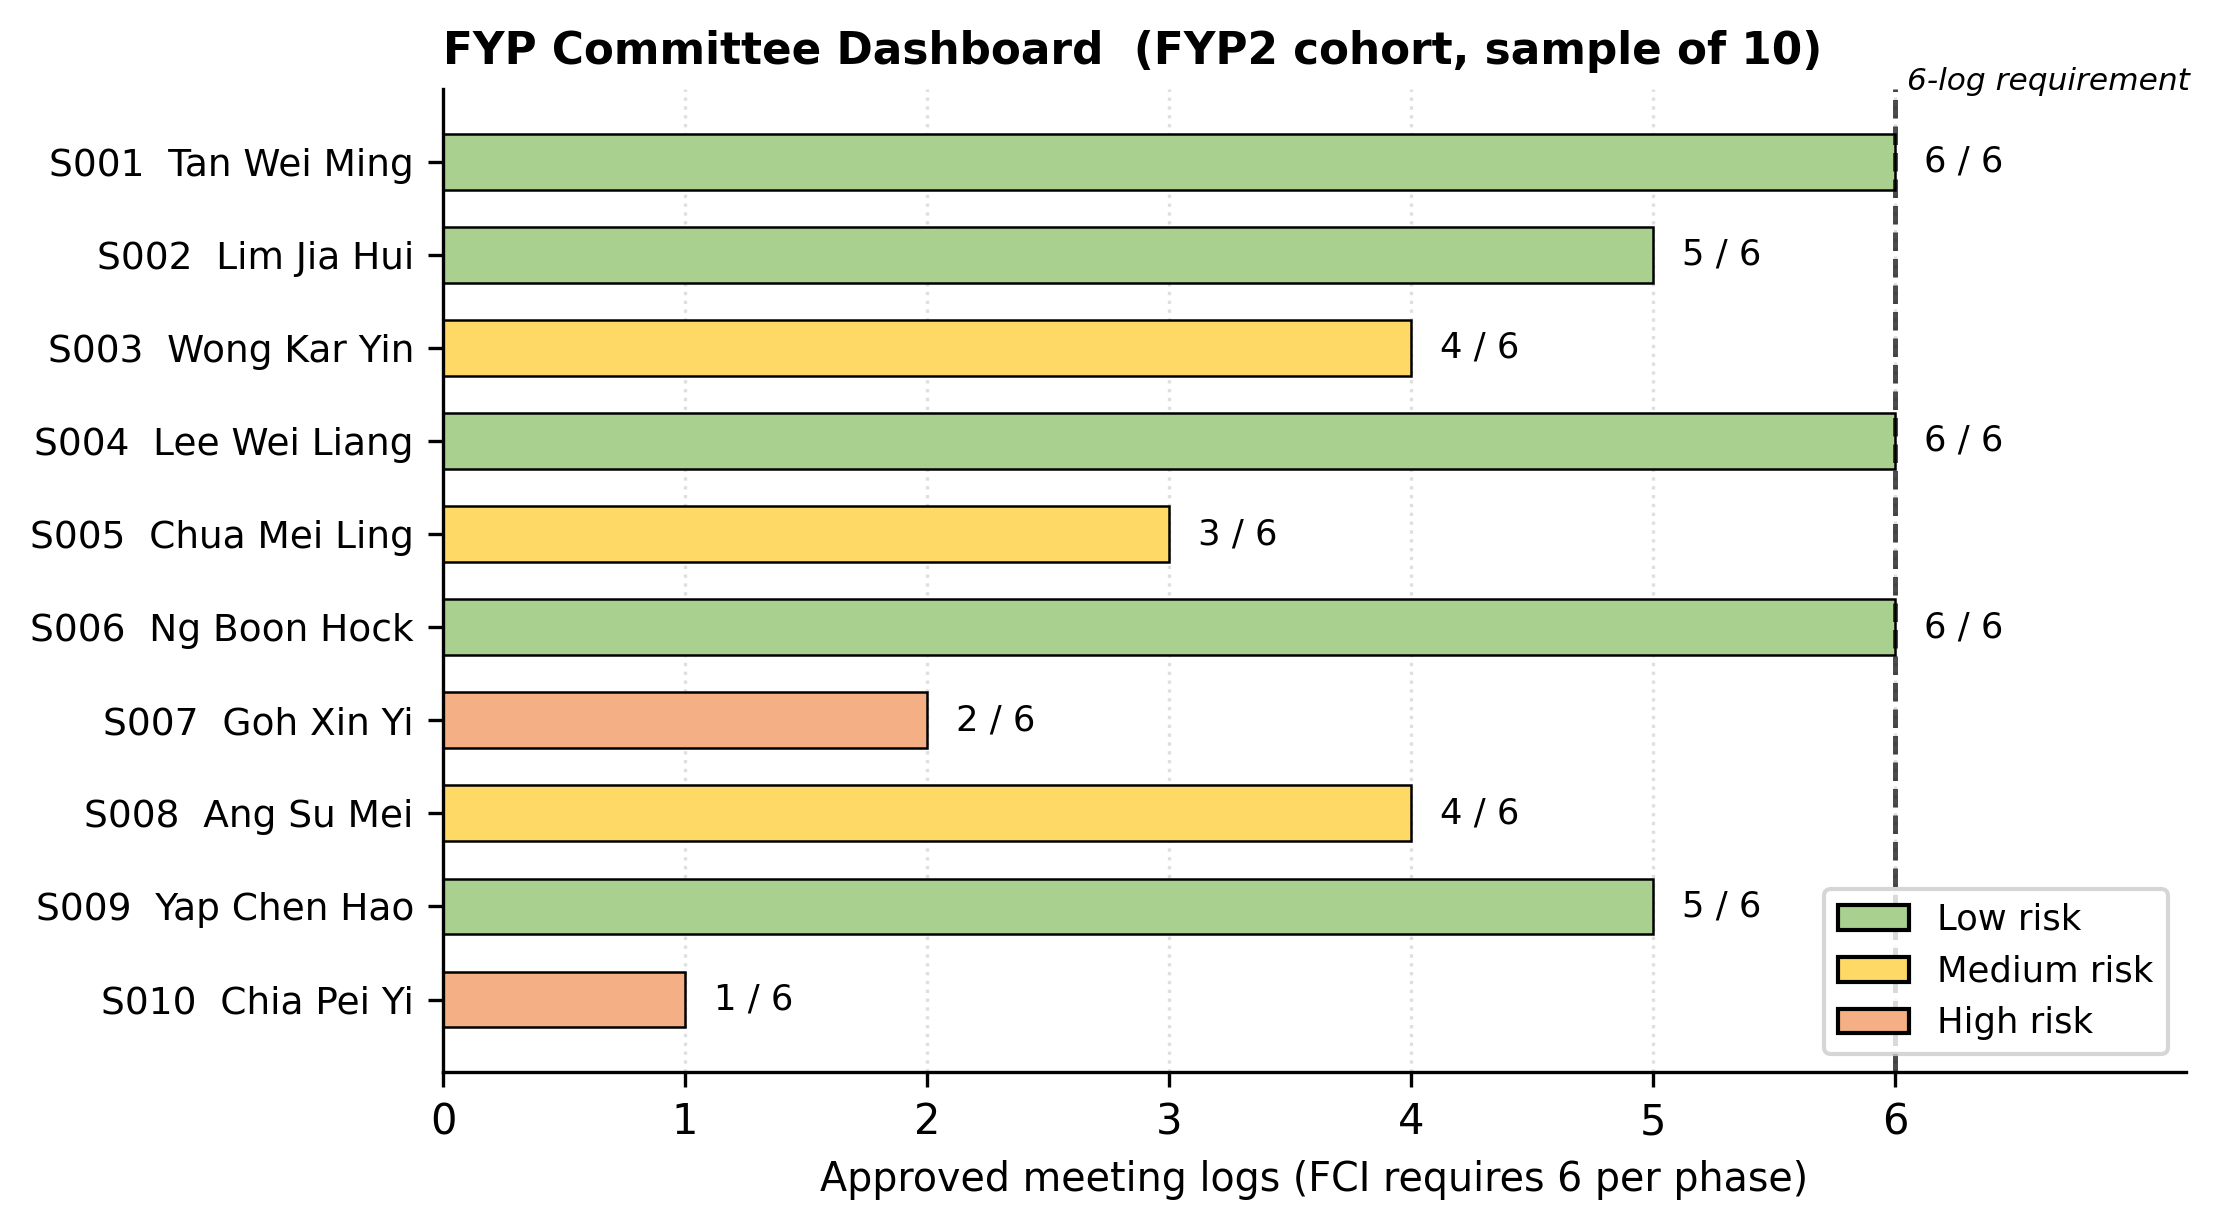
\includegraphics[width=\columnwidth]{fig5-committee-dashboard.png}
\caption{Committee dashboard for an FYP2 cohort of 37 students. Each row represents one supervisee. Risk colouring (red, amber, green) is computed from meeting log compliance, recency of last meeting, and time elapsed since pairing. The Export CSV button on the top right downloads the full cohort table in the format the faculty office currently pastes into its existing spreadsheet.}
\label{fig:dashboard}
\end{figure}

\section{Discussion}

\subsection{What Worked Well}
The widest piece of value is the coverage across all four roles. Many student projects in this space build the student side and hand-wave the rest. Building the supervisor side, the committee side and the admin side adds a lot of work but the resulting product feels usable to all four parties rather than just one.

The three-AI-service split, rather than a single hosted-LLM wrapper, turned out to be the right call in retrospect. Each service is accountable to a narrower task. The supervisor recommender is deterministic and can be explained to a student in plain words. The proposal analyser produces five structured scores rather than free-form prose, which is easier for students to act on. The chatbot is grounded in the FCI handbook through retrieval, which reduces the likelihood of hallucinated answers.

The signed meeting log is the strongest compliance feature. The SHA-256 hash in the footer makes the exported DOCX self-verifying. The FCI letterhead is preserved so the output can replace the existing paper sheet without changing the moderation pipeline. Apache POI's run-splitting behaviour made the renderer harder to build than expected but the end result is reliable.

\subsection{What Did Not Work as Smoothly}
Schema migrations bit harder than expected. Flyway treats every applied migration as immutable. A typo in V15 was found while V20 was already in the database, and the only way to fix the typo was to write a corrective V21 rather than edit V15. This is an obvious rule once you have hit it once but it was not obvious before. The project carries 39 migrations now, with V29 deliberately skipped after an earlier checksum collision.

The first version of the meeting log renderer passed every JUnit case but produced files that Word refused to open. The cases were inspecting the XML directly rather than opening the produced bytes with \texttt{XWPFDocument} and looking at what a reader would see. Adding end-to-end cases that mimicked the reader's view caught the bug and several similar ones afterwards. This shifted the project's testing discipline: tests now check the artefact the user sees, not just the intermediate representation.

\subsection{Limitations}
Two non-functional requirements were left for deployment. NFR7 (uptime above ninety-nine per cent) and NFR8 (scheduled backups) are running-system properties rather than build-time ones, and the production deployment behind the MMU TLS proxy was outside the scope of FYP2. The UI is English-only. The acceptance testing sample is small. The system has not been load-tested at the scale of a full one-thousand-student cohort.

\section{Conclusion and Future Work}
The system delivers what the FYP2 objectives asked for. Four user roles are supported. Three AI services run independently. Meeting logs are dual-signed and exported. The trimester cycle is modelled as a real entity with read-only gating. Testing across five layers returned no failures, and acceptance was signed off for each user role.

What remains is mostly operational and incremental. Three groups of future work are planned.

The first group is operational: deploy behind the MMU TLS proxy, wire the backup endpoint to a weekly cron, and stand up an uptime dashboard.

The second group is feature extension. A read-only audit log viewer for the administrator. Single sign-on against the institutional identity provider. Multi-language support for Bahasa Malaysia and Mandarin. A cohort statistics dashboard that builds on the committee report.

The third group is research extension. A larger pilot study at the scale of a full faculty cohort. A head-to-head comparison between the deterministic recommender and a hosted large-language-model recommender, to see whether deterministic explainability is worth the loss of generality. An investigation into whether the meeting log subsystem can be generalised to postgraduate thesis supervision, where the compliance audit trail matters even more.

The broader lesson from the project is that purpose-built domain tools can outperform general productivity stacks even when the general stacks are already paid for. The gap is widest where compliance, audit and AI assistance meet a workflow that the incumbents do not target.

\section*{Acknowledgements}
The author thanks the FCI project supervisor for guidance through both FYP1 and FYP2, the testers from each user role for the time they gave to the usability and acceptance sessions, and the classmates who suffered through early demo builds and reported the bugs that the JUnit suite missed.

\begin{thebibliography}{00}
\bibitem{smith2021} A. K. Smith and L. R. Patel, ``Adapting learning management systems for one-to-one academic supervision: a case study,'' in \emph{Proc. Int. Conf. on Engineering Education}, Kuala Lumpur, Malaysia, 2021, pp. 145 to 152.

\bibitem{tan2022} R. Tan and B. Lim, ``Limitations of course-based platforms for final-year project supervision,'' \emph{Journal of Educational Technology Systems}, vol. 50, no. 3, pp. 312 to 329, 2022.

\bibitem{wang2018} H. Wang, F. Chen and X. Liu, ``Collaborative filtering for academic advisor recommendation,'' in \emph{Proc. ACM Conf. on Recommender Systems}, Boston, USA, 2018, pp. 412 to 420.

\bibitem{reimers2019} N. Reimers and I. Gurevych, ``Sentence-BERT: sentence embeddings using siamese BERT networks,'' in \emph{Proc. Conf. on Empirical Methods in Natural Language Processing}, Hong Kong, 2019, pp. 3982 to 3992.

\bibitem{ramesh2022} D. Ramesh and S. Sanampudi, ``An automated essay scoring systems: a systematic literature review,'' \emph{Artificial Intelligence Review}, vol. 55, no. 3, pp. 2495 to 2527, 2022.

\bibitem{lewis2020} P. Lewis et al., ``Retrieval-augmented generation for knowledge-intensive NLP tasks,'' in \emph{Advances in Neural Information Processing Systems}, vol. 33, Vancouver, Canada, 2020, pp. 9459 to 9474.

\bibitem{sanh2019} V. Sanh, L. Debut, J. Chaumond and T. Wolf, ``DistilBERT, a distilled version of BERT: smaller, faster, cheaper and lighter,'' in \emph{Proc. NeurIPS Workshop on Energy Efficient Machine Learning and Cognitive Computing}, Vancouver, Canada, 2019, pp. 1 to 5.

\bibitem{johnson2021} J. Johnson, M. Douze and H. Jegou, ``Billion-scale similarity search with GPUs,'' \emph{IEEE Transactions on Big Data}, vol. 7, no. 3, pp. 535 to 547, 2021.

\bibitem{mqa2018} Malaysian Qualifications Agency, \emph{Code of Practice for Programme Accreditation (Engineering and Engineering Technology)}, 2nd ed., Petaling Jaya, Malaysia: MQA, 2018.

\bibitem{martin2017} R. C. Martin, \emph{Clean Architecture: A Craftsman's Guide to Software Structure and Design}. Boston, USA: Prentice Hall, 2017.
\end{thebibliography}

\end{document}
